\documentclass[12pt,a4paper]{article}

\input{../preamble_files/packages}
\input{../preamble_files/figures}
\input{../preamble_files/references}
\input{../preamble_files/shortcuts}

\pagestyle{fancy}
\lhead{Richard Whitehill}
\chead{MATH 513 -- HW 4}
\rhead{02/20/22}
\cfoot{\thepage~of~\pageref{LastPage}}

\newcommand{\prob}[2]{\textbf{#1)} #2}
\newenvironment{proof}
{
\textbf{\underline{Proof}} \\
}
{
\begin{flushright}
$\blacksquare$
\end{flushright}}

\setlength{\parskip}{\baselineskip}
\setlength{\parindent}{0pt}

\begin{document}

\prob{1}{Compute the order of each element in the dihedral group $D_6$ and $D_8$.}

$\rightarrow$ Consider the symmetries of a triangle given in the figure below and let $D_6 = \{R_{0},R_{60},\\ R_{120},D_1,D_2,D_3\}$. 
\bef
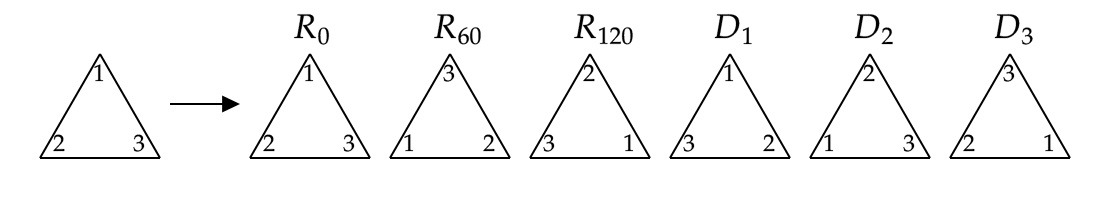
\includegraphics[scale=0.3]{fig1.png}
\eef

Then we have the following
\begin{table}[H]
 \begin{center}
  \begin{tabular}{|c|c|c|c|c|c|c|}
   \hline
   element & $R_{0}$ & $R_{60}$ & $R_{120}$ & $D_1$ & $D_2$ & $D_3$ \\
   \hline
   order & 1 & 3 & 3 & 2 & 2 & 2 \\
   \hline
  \end{tabular}
 \end{center}
\end{table}
For each symmetry operation, we consider the minimum number of applications that are needed to return to the original configuration. Obviously, $R_{0}$ is the identity, which always has order of 1 for any group, and the reflections across diagonals through the vertices and center must be performed twice.

Now consider the symmetries of a square shown below and let $D_8 = \{R_{0},R_{90},R_{180},R_{270},H,\\V,D,D'\}$. 
\bef
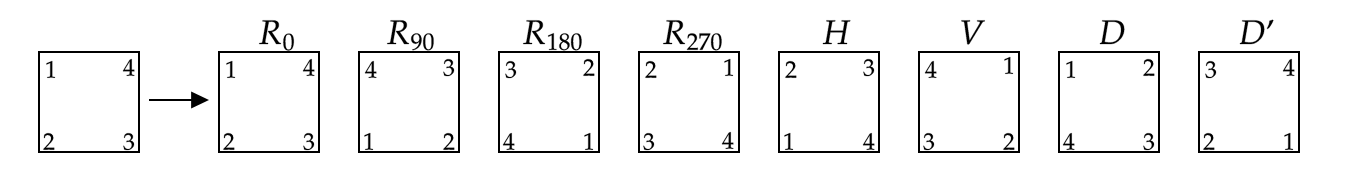
\includegraphics[scale=0.3]{fig2.png}
\eef

Then it follows that
\begin{table}[H]
 \begin{center}
  \begin{tabular}{|c|c|c|c|c|c|c|c|c|}
   \hline
   element & $R_{0}$ & $R_{90}$ & $R_{180}$ & $R_{270}$ & $H$ & $V$ & $D$ & $D$ \\
   \hline
   order & 1 & 4 & 2 & 4 & 2 & 2 & 2 & 2 \\
   \hline
  \end{tabular}
 \end{center}
\end{table}

\prob{2}{Show that $\left<a,b | a^2=b^2=(ab)^2=\id \right>$ give a presentation for $D_{2n}$ in terms of the two generators $a = s$ and $b = sr$ of order $2$.}

The dihedral group in terms of the rotation and reflection generators $r,s$ is given as 
\begin{align*}
D_{2n} = \langle r,s | r^{n} = s^2 = \id,~rs=sr^{-1} \rangle
\end{align*}
We show that the representation above holds for $n = 2$.

\begin{proof}
First, we prove that the representation in terms of $a,b$ implies the relations for the representation in terms of $r,s$. First, notice that $a^2 = s^2 = \id$ and $(ab)^2 = (ssr)^2 = (s^2r)^2 = r^2 = \id$. Next, we see that $b^2 = (sr)^2 = \id$, $sr = r^{-1}s$, and $rs = sr^{-1}$.

Now, we prove that the representation in terms of $r,s$ implies the relations for the representation in terms of $a,b$. Observe $s^2 = a^2 = \id$ and $r^2 = (ab)^2 = \id$. Finally, notice that $rs = sr^{-1}$ or $(sr)^2 = b^2 = \id$.
\end{proof}

\prob{3[1.1.1]}{Complete the multiplication table for $D_8$. Find at least one interesting pattern in the table.}

\begin{table}[H]
 \begin{center}
  \begin{tabular}{c|cccccccc}
    & $R_{0}$ & $R_{90}$ & $R_{180}$ & $R_{270}$ & $H$ & $V$ & $D$ & $D'$ \\
  \hline
  $R_{0}$ & $R_{0}$ & $R_{90}$ & $R_{180}$ & $R_{270}$ & $H$ & $V$ & $D$ & $D'$ \\ 
  $R_{90}$ & $R_{90}$ & $R_{180}$ & $R_{270}$ & $R_{0}$ & $D'$ & $D$ & $H$ & $V$ \\
  $R_{180}$ & $R_{180}$ & $R_{270}$ & $R_{0}$ & $R_{90}$ & $V$ & $H$ & $D'$ & $D$ \\
  $R_{270}$ & $R_{270}$ & $R_{0}$ & $R_{90}$ & $R_{180}$ & $D$ & $D'$ & $V$ & $H$ \\
  $H$ & $H$ & $D$ & $V$ & $D'$ & $R_{0}$ & $R_{180}$ & $R_{90}$ & $R_{270}$ \\
  $V$ & $V$ & $D'$ & $H$ & $D$ & $R_{180}$ & $R_{0}$ & $R_{270}$ & $R_{90}$ \\
  $D$ & $D$ & $V$ & $D'$ & $H$ & $R_{270}$ & $R_{90}$ & $R_{0}$ & $R_{180}$ \\
  $D'$ & $D'$ & $H$ & $D$ & $V$ & $R_{90}$ & $R_{270}$ & $R_{180}$ & $R_{0}$ \\
  \end{tabular}
 \end{center}
\end{table}

One interesting thing to note is that there are distinct quadrants of product transformations. For products of rotations and reflections we get effectively rotations, which are shown in the upper left and lower right corners. However when the product contains one reflection and one rotation we get reflections effectively, shown in the lower left and upper right corners.

\prob{4[1.1.4]}{}

(a) List the symmetries of a rectangle.

The symmetries are given in the second figure in problem 1 and can be put into the set $D_8$, which is also given in problem 1.

(b) Write the multiplication table for the symmetries of a rectangle.

The multiplication table for the symmetries of a rectangle are shown in the multiplication table in problem 3.

\prob{5[1.1.5]}{}

(a) Find the center of $D_8$

The center of a group $G$ is the set of all elements $a \in G$ such that $ab = ba$ for all $b \in G$ (i.e. $a$ commutes with all elements of $G$). We can read from the table in problem 3 what elements are in the center of $D_8$:
\begin{align*}
\mathbf{Z}(D_8) = \{R_0,R_{180}\}
\end{align*}

(b) Find $\mathbf{C}_{D_8}(R_{90})$ and $\mathbf{C}_{D_8}(H)$.

The centralizer of an element $a \in G$ is the set of all elements $b \in G$ such that $a$ and $b$ commute:
\begin{align*}
\mathbf{C}_{D_8}(R_{90}) = \{R_{0},R_{90},R_{180},R_{270}\}
\end{align*}
\begin{align*}
\mathbf{C}_{D_8}(H) = \{H,R_{180},R_{0},V\}
\end{align*}

\prob{6[1.1.6]}{Let $D_6$ denote the set of symmetries of an equilateral triangle. Find the multiplication table for $D_6$. What is the center of $D_6$?}

\begin{table}[H]
 \begin{center}
  \begin{tabular}{c|cccccc}
   & $R_{0}$ & $R_{60}$ & $R_{120}$ & $D_1$ & $D_2$ & $D_3$ \\
  \hline
  $R_{0}$ & $R_{0}$ & $R_{60}$ & $R_{120}$ & $D_1$ & $D_2$ & $D_3$ \\
  $R_{60}$ & $R_{60}$ & $R_{120}$ & $R_{0}$ & $D_2$ & $D_3$ & $D_1$ \\
  $R_{120}$ & $R_{120}$ & $R_{0}$ & $R_{60}$ & $D_3$ & $D_1$ & $D_2$ \\
  $D_1$ & $D_1$ & $D_3$ & $D_2$ & $R_{0}$ & $R_{120}$ & $R_{60}$ \\
  $D_2$ & $D_2$ & $D_1$ & $D_3$ & $R_{60}$ & $R_{0}$ & $R_{120}$ \\
  $D_3$ & $D_3$ & $D_2$ & $D_1$ & $R_{120}$ & $R_{60}$ & $R_{0}$ \\
  \end{tabular}
 \end{center}
\end{table}

\prob{7[1.2.4]}{Let $\sigma = (1~3~5)(2~4)$ and $\tau = (1~5)(2~3)$ be elements of $S_5$. Find $\sigma^2$, $\sigma\tau$, $\tau\sigma$, and $\tau\sigma^2$.}

\begin{alignat*}
\sigma \sigma^2 &= [(1~3~5)(2~4)][(1~3~5)(2~4)] &&= (1~5~3) \\
\sigma\tau &= [(1~3~5)(2~4)][(1~5)(2~3)] &&= (5~3~4~2) \\
\tau\sigma &= [(1~5)(2~3)][(1~3~5)(2~4)] &&= (1~2~4~3) \\
\tau\sigma^2 &= [(1~5)(2~3)](1~5~3) &&= (5~2~3)
\end{alignat*}

\prob{8[1.2.5]}{Construct a complete multiplication table for $S_3$. What is the center of $S_3$? If $f = (1~2~3)$, what is $\mathbf{C}_{S_3}(f)$, the centralizer of $f$ in $S_3$?}

$\rightarrow$ We know that $S_3 = {\rm Perm}(\{1,2,3\}) = \{\id,(2~3),(1~2),(1~2~3),(1~3~2),(1~3)\}$. Hence,
\begin{table}[H]
 \begin{center}
  \begin{tabular}{c|cccccc}
   & $\id$ & (2~3) & (1~2) & (1~2~3) & (1~3~2) & (1~3) \\
  \hline
  $\id$ & $\id$ & (2 3) & (1 2) & (1 2 3) & (1 3 2) & (1 3) \\
  (2 3) & (2 3) & $\id$ & (1 3 2) & (1 3) & (1 2) & (1 2 3) \\
  (1 2) & (1 2) & (1 2 3) & $\id$ & (2 3) & (1 3) & (1 3 2) \\
  (1 2 3) & (1 2 3) & (1 2) & (1 3) & (1 3 2) & $\id$ & (2 3) \\
  (1 3 2) & (1 3 2) & (1 3) & (2 3) & $\id$ & (1 2 3) & (1 2) \\
  (1 3) & (1 3) & (1 3 2) & (1 2 3) & (1 2) & (2 3) & $\id$ \\
  \end{tabular}
 \end{center}
\end{table}

and 
\begin{align*}
\mathbf{C}_{S_3}(f) = \{\id,(1~2~3),(1~3~2)\}
\end{align*}

\prob{9[1.2.6]}{Let $f = (1~2~3) \in S_3$. Find the maps in the following sequence
\begin{align*}
\id_{[3]},f,f^2,f^3,f^4,f^5,\hdots
\end{align*}
Do you see a pattern?}

Notice that from the table we see that
\begin{align*}
f^{0} &= \id_{[3]} \\
f^{1} &= (1~2~3) \\
f^{2} &= (1~2~3)(1~2~3) = (1~3~2) \\
f^{3} &= (1~2~3)(1~3~2) = \id_{[3]} \\
\vdots
\end{align*}
It is seen that this sequence essentially lists the elements of the cyclic group $\langle f \rangle = \{f,f^2,f^3=\id_{[3]}\}$.


\end{document}
